\documentclass[12pt]{article}

% fonts

\usepackage{pdflscape}
\usepackage[T1]{fontenc}
\usepackage[full]{textcomp}
\usepackage{newtxtext}
\usepackage{cabin} % sans serif
\usepackage[varqu,varl]{inconsolata} % sans serif typewriter
\usepackage[final,expansion=alltext]{microtype}
\usepackage[english]{babel}
\usepackage{amsmath}
\usepackage[bigdelims,vvarbb]{newtxmath} % bb from STIX
\usepackage[cal=boondoxo]{mathalfa} % mathcal
\usepackage{csquotes}
\usepackage{graphicx}
\usepackage{hyperref}
\usepackage{indentfirst}

\usepackage[backend=bibtex,style=numeric]{biblatex}
\bibliography{traffic} % Specify your BibTeX file

% geometry of the page

\usepackage[top=1in,
            bottom=1in,
            left=1in,
            right=1in]{geometry}


% paragraph spacing

\setlength{\parindent}{24pt}
\setlength{\parskip}{1ex plus 0.4ex minus 0.2ex}


\author{Matthew McAnear}
\title{The Effect of Advanced Safety Features on Crash Fatality Rates for Vulnerable Road Users}

% useful packages

\begin{document}

\maketitle

\begin{abstract}
    Over the past several decades, cars in the United States have continued to grow larger. For drivers, these cars
    have also increased in safety compared to earlier models, with new advanced saftey features becoming more
    commonplace in all vehicles. Despite the proliferation of AI technology in passenger cars for collision
    detection/avoidance, lane drift systems, and various other safety systems, we find that these systems do not
    show significant reductions in the risk of fatalities for pedestrians and cyclists in single-vehicle accidents. The
    results are somewhat ambiguous, but it appears that the overall fatality rate for vulnerable road users is driven
    by the size and weight of vehicles, lighting conditions, and region more than advanced safety features can offset.
\end{abstract}


\section{Introduction}

The National Highway Traffic Safety Administration (NHTSA) reports that, as of preliminary reports through
June of 2023, traffic accidents involving fatalities, in aggregate, are down about 3\%. This decrease is positive,
but looking only at changes from year to year hides the true scale of the problem for vulnerable non-vehicle
road users. While the overall change for pedestrians is also 3\%, the baseline level of risk for pedestrians is
much higher than for passenger vehicles or even for pedalcyclists. Among accidents involving pedestrians, the fatality
range anywhere from a 14\% to 23\% baseline fatality rate throughout the year, depending on the month in
question \cite{national_highway_traffic_safety_administration_early_2024}.

This fatality rate is influenced heavily by the mass of the car\cite{evans_car_1992}. This means that there
are offsetting effects of both increasing vehicle mass and increasing
vehicle saftey. For people outside of the vehicle, however, the statistics are alarming. According to Tyndall,
"between 2010 and 2021 the number of pedestrians killed annually in collisions increased by 72\%, from 4300 to
7400 \cite{tyndall_effect_2024}." Due to relaxed emissions standards for small trucks compared to passenger cars,
American buyer preferences shifted toward sport utility vehicles (SUVs) and trucks \cite{kovach_rise_2021}. Taken into
account this connection between both the proliferation of large vehicles and the clear connection in fatality risk to
more massive and taller vehicles\cite{tyndall_effect_2024}, finding the factors that minimize pedestrian fatalities
is of critical importance for public health.

It is common knowledge that AI systems have become an increasing part of every day life, and passenger
vehicles are no exception. The question is if these improved safety systems are reducing the risk of fatalities
among pedestrians and cyclists. Next, assuming these new systems yield tangible improvements to pedestrian safety,
are the improvements large enough in magnitude to offset the increased risk from the size and height of vehicles?

In this paper, we focus primarily on those factors that influence the risk of fatalities in crashes involving pedestrians
and cyclists. After controlling for the effect of weather conditions,
geographic region, and crash variables such as time of day and intersection type, we estimate the effect
of advanced safety features on the risk of pedestrian and cyclist fatalities within vehicle types. We hypothesize
that advanced safety feature have limited effects on crash fatality, and that the size and weight of the vehicle are 
the most important predictors of crash fatality. All code used in the analysis and data cleaning steps is available on
\url{https://github.com/mcanearm/road_fatilities}


\section{Data}

Our data comes from the US National Highway Traffic Safety Administration (NHTSA). The NHTSA collects and distributes
crash statistics on fatal accidents through FARS, the Fatal Accident Reporting System, and CRSS, the Crash Report
Sampling System. Through these two datasets, we can investigate risk factors for fatal accidents and injuries in
pedestrian and cyclist accidents. All files are available at
    [the NHTSA website](https://www.nhtsa.gov/file-downloads?p=nhtsa/downloads/).  Fatal accidents and non-fatal 
accidents are reported through two separate systems, and care must be taken when combining the two sources. For example,
the CRSS data is taken from 60 sampling locations, not nationwide, and weights are applied in order to estimate 
national level statistics\cite{national_highway_traffic_safety_administration_crash_nodate}. We will use these weights
in our estimation. 

To simplify the analysis, we exclude from consideration crashes involving multiple vehicles and focus solely 
on single-vehicle collisions with pedestrians and cyclists. We also further ignore the crash group, i.e. 
whether the driver or cyclist was at fault, what specific maneuver was being performed, or where the pedestrian/cyclist
was in relation to the vehicle. These are important characteristics to consider, but the overall sparsity of the data 
makes inference in small subgroups challenging. We utilize the \texttt{scikit-learn} package for data preprocessing,
specifically to create one-hot encodings of nearly all features\cite{pedregosa_scikit-learn_2011}.

Another potential issue with the dataset is the overall level of sparsity in our features. While there is no
missingness for important crash level statistics such as the bodyclass of the vehicle, things like the weight class
are missing and cannot be reliably imputed\footnote{
    Weight class is tied to the individual car, so the median would not work in this case. The appropriate rememdy would be to  
    find the weight from the manufacturer of the vehicle for the listed options package, if available, but this is quite 
    tedious and it is unclear that it would yield improvements to our analysis.}. 
Safety features are also missing for a large number of vehicles; to solve
this, we assume that any safety feature not listed as "standard" is not present. Though we could simulate this data
conditional on other factors, this is an extension to a future analysis and out of scope for this short paper. It is 
also a clear and fundamental limitation of the dataset we are using, as there is a contradictive relationship between
the weight of the vehicle, its price, and therefore its included safety features. If more dangerous cars are more loaded
with safety features, it could appear that the safety features are the reason for the increased fatality rate, and so
we must proceed with caution.

\section{Methodology}

We utilize a logistsic regression model, as we are primarily interested in inference on the
effects of our variables of interest and so require a model that retains interpretability. However, we will
add hierarchical structure to account for both the full and group-level effects of each covariate across
cyclists and pedstrians. See Figure \ref{fig:model_graph} for a graphical representation of the model. For safety
features in particular, we choose a choose a relatively small subset of the available features that seem 
\textit{a priori} to be most relevant to preventing outcomes. 

We wish to estimate the effects of the variables separately for both pedestrians and cyclists, but because of our
relatively sparse feature space, there is some concern of wild coefficient values, so for that reason we use the
hierarchical model to constrain an overall effect of a feature, and then estimate whether that effect differs
between cyclists and pedestrians. The overall effects considered are vehicle type (bodyclass), lighting and weather
(i.e. environmental) conditions, and vehicle safety features. Each beta coefficient is assumed to follow a Normal prior. 
We re-use the variability nuisance parameter for multiple levels of the hierarchy, as this simplified model fitting and 
prevented divergences in the sampling process, though it may be a source of bias in our estimates.

To control feature sparsity, we also introduce latent discrete variables for whether to include a particular
variable in the regression model. Our posterior estimates of these variables will give us a sense of which features
are worth including in the regression, as well as their final effect on the outcome. This allows us to mimic the
Bayesian Model averaging functionality of the \texttt{BMA}\cite{raftery_bma_2022} using our model specification in
Numpyro\cite{phan_composable_2019} along with our hierarchical model structure. This model averaging approach sounds
similar in theory to using Laplace priors as specified by Tibshirani in \cite{tibshirani_regression_1996},
but after trying both methods, the two results are quite different in practice. We will opt to use the model
averaging approach, as this allows to better handle sparsity and yields a more parsimonious model.
Our prior predictive check (Figure \ref{fig:ppc}) shows that this model is not overly specific and can capture the
range of outcomes we are interested in.

\section{Results}

The overall fatality rate in accidents varies distinctly by region and vulnerable road user
type (pedestrian or cyclist). As shown in \ref{fig:prob_intercepts}, the overall fatality rate
among cyclists, irrespective of region, is only about 1\%, holding all other things constant. Surpsingly,
there is a clear relationship between the fatality rate and the region, with pedestrians in the West, Midwest, and South
subject to significantly higher fatality rates in accidents when compared to the Northeast. This may likely
be due to an overall lower incidence of vehicles in the Northeast, more options for transportation away from roadways
in major urban areas, and lower speeds in highly congested cities that are not present in other regions to the
same degree.

Many of the results are exactly as one would expect, and partially align with our hypothesis. For example, the
coefficient on pickup trucks is strongly positive for both cyclists and for pedestrians, indicating that these vehicles
are much more likely to kill a pedestrian or cyclist compared to cars (the baseline group). See
Figure \ref{fig:coefficients}. Many results border on the obvious - the log-odds of a fatality increase the most when
a truck/semi are involved. The trend genereally holds that increasing vehicle weight and size corresponds to an increasing
likelihood of fatality for pedestrians and cyclists. Somewhat surprising is how these effects are manifested across
vulnerable road users. For example, pickups and semis are much more likely to kill a cyclist than a pedestrian. This is
most likely due to the nature of when and where cycling accidents take place, presumably at higher speeds on shared
infrastructure. Unfortunately, the data are missing vehicle speed in roughly 58\% of the accidents in our data, and so
use of this as a control variable may unfairly bias our results without a more thoughtful imputation scheme.

Outside of the vehicle centric effects, the largest effects is by far if the accident takes place at night, shown in
figures \ref{fig:coefficients} and \ref{fig:all_users}. This effect is roughly the same for pedestrians and cyclists.
Inclement weather appears to have a negative effect, such that
worse weather actually reduces the log odds of a fatality. This could be due to drivers being more cautious in
inclement weather, and also because we have collapsed a large variety of weather conditions into a single variable.

Still, controlling for these factors, it appears that our safety features have relatively small or unclear effects on
the log-odds of a fatality. A marginal effect for pedestrian auto braking may be present for pedestrians, but it pales
in comparison to the overall magnitude of effect of vehicle size and lighting conditions.
The clearest effect is the lane-departure warning system, which appears to reduce the
log-odds of a fatality substantially among cyclists. Equally substantially, however, is the effect of lane-keeping
assistance features, which appears to \textit{increase} the log-odds of a fatality among cyclists.

To make sense of these counterintuitive result, we should remember that the sparsity and high-proportion of missingness
in our data inherently means that certain subgroups of the data will suffer from multicollinearity that biases
our coefficient estimation. Next, recall that all estimates are based on sampling weights derived by the NHTSA, and if
these weights are improperly calibrated after filtering certain accidents, we could be biasing our results.
We also see evidence for this in the inclusion probabilities of our features, as shown in 
Figure \ref{fig:inclusion_probs}. While several features have high inclusion probabilities that make practical sense, 
the exclusion of SUVs but the inclusion of pickups, despite their similarity, is cause for concern, and we are 
justified in disregarding this finding through invocation of Occam's razor until further analysis is conducted.

Further proof of this can be found in our posterior predictive checks. We notice immediately that our overall fatality
rate estimated by the model is lower than than what is reported as of the preliminary results for 2024 by the NHTSA. 
The most likely explanation is that the dataset, as we've subsetted
it, has systematically lower fatality rates than the overall dataset. The exclusion of accidents
with multiple vehicles may be the culprit, as it is reasonable to suppose these accidents to involve
multiple vehicles because they are higher speed and more dangerous. The distribution of our probabilities follows
a multimodal shape, and this is to be expected given the sharp differences across regions
and pedestrian types (see Figure \ref{fig:prob_dist}). Lastly, we may examine an estimated $R^2$ as outlined by
Gelman et. al\cite{gelman_r-squared_2019} in Figure \ref{fig:r2_dist}. We see that no matter how we choose to interpret
our findings, the reality is that the total variance explained by our data is well under 10\%, indicating missing factors
from the analysis. Most notably, this is probably items such as crash group, vehicle
speed, intersection type or roadway location, and other factors that are not included in our anlaysis for reasons
of missingness or complexity, but are nontheless potentially more predictive than the values we have selected.

\section{Conclusion}

Before making any sweeping conclusions, we should interpret our model results cautiously. In particular, the CRSS
data used requires correctly specifying the weights for the sampling locations, yet these weights may need to be
recalibrated prior to their use in our model for more accurate results. We have not utilized any particular
survey methodology in our model and estimation procedure. Further, there are clear signs of model mis-specification
based on the posterior distribution of several of our coefficient estimates when compared against our prior idea of what
the effects should be, especially in the cases of SUVs and lane-keeping assistance features. For the same reason tht we
excluded alcohol involvement from our analysis, we potentially should have excluded some safety features with high 
sparsity.

There is a philosophical issue with this analysis which is unavoidable; we can only model 
observed accidents, and by definition, accidents prevented by advanced safety features are not included
as in the model. Therefore, we must rely on a time-series and causal analysis to be more
sure whether we have properly estimated the effects of these features, and this remains a future area of
research.

Nevertheless, we have shown that the overall fatality rate for pedestrians and cyclists in single-vehicle car
crashes can be partially explained by several factors, some of which align with our initial hypothesis and
some that do not. The involvement of a pickup truck and poor lighting conditions are important factors
when predicting whether a particular accident may be fatal for folks outside the vehicle, but SUVs have no practical
significance as estimated by the model, and crossover vehicles actually decrease the probability of a fatal accident
as compared to cars. Region is also a significantly more important predictor of fatality than we initially supposed.

Once accounting for our environmental and vehicle-centric features, we find that the overall impact
of advanced safety features is marginal at best, and evidence for their effectiveness
can be contradictory. Region, vehicle size, and environmental conditions play a much
larger role in the fatality of crashes than the presence or absence of safety features, and this research
shows no unambiguous evidence that adding these features to large vehicles such as pickups
and work vehicles will reduce the fatality rates for vulnerable road users in any practical sense.

\section{Support}

\begin{figure}[h]
    \centering
    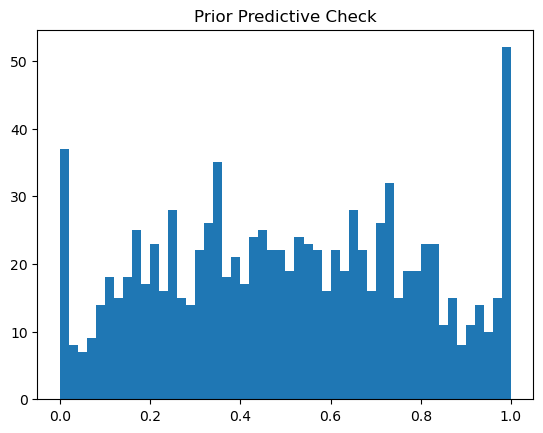
\includegraphics[width=\textwidth]{images/prior_predictive_check.png}
    \caption{Prior predictive check for the model. We are getting a multimoddal distribution, but we
        also have a relatively complicated model. We are predicting probabilities on the entire
        range from 0 to 1, so we can be reasonably confident that our model is as flexible as required.}
    \label{fig:ppc}
\end{figure}

\begin{figure}[h]
    \centering
    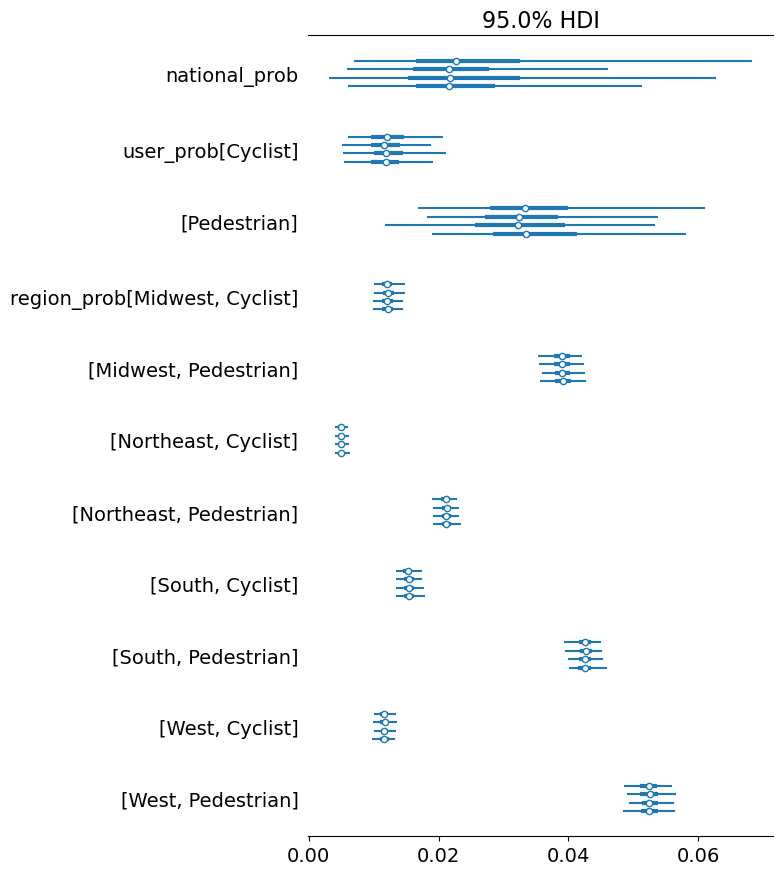
\includegraphics[width=\textwidth]{images/prob_intercepts.png}
    \caption{Forest plot of each group-level intercept. The intercepts are fit on log-odds,
        but converted to probabilities for this plot.}
    \label{fig:prob_intercepts}
\end{figure}


    \begin{figure}[h]
        \centering
        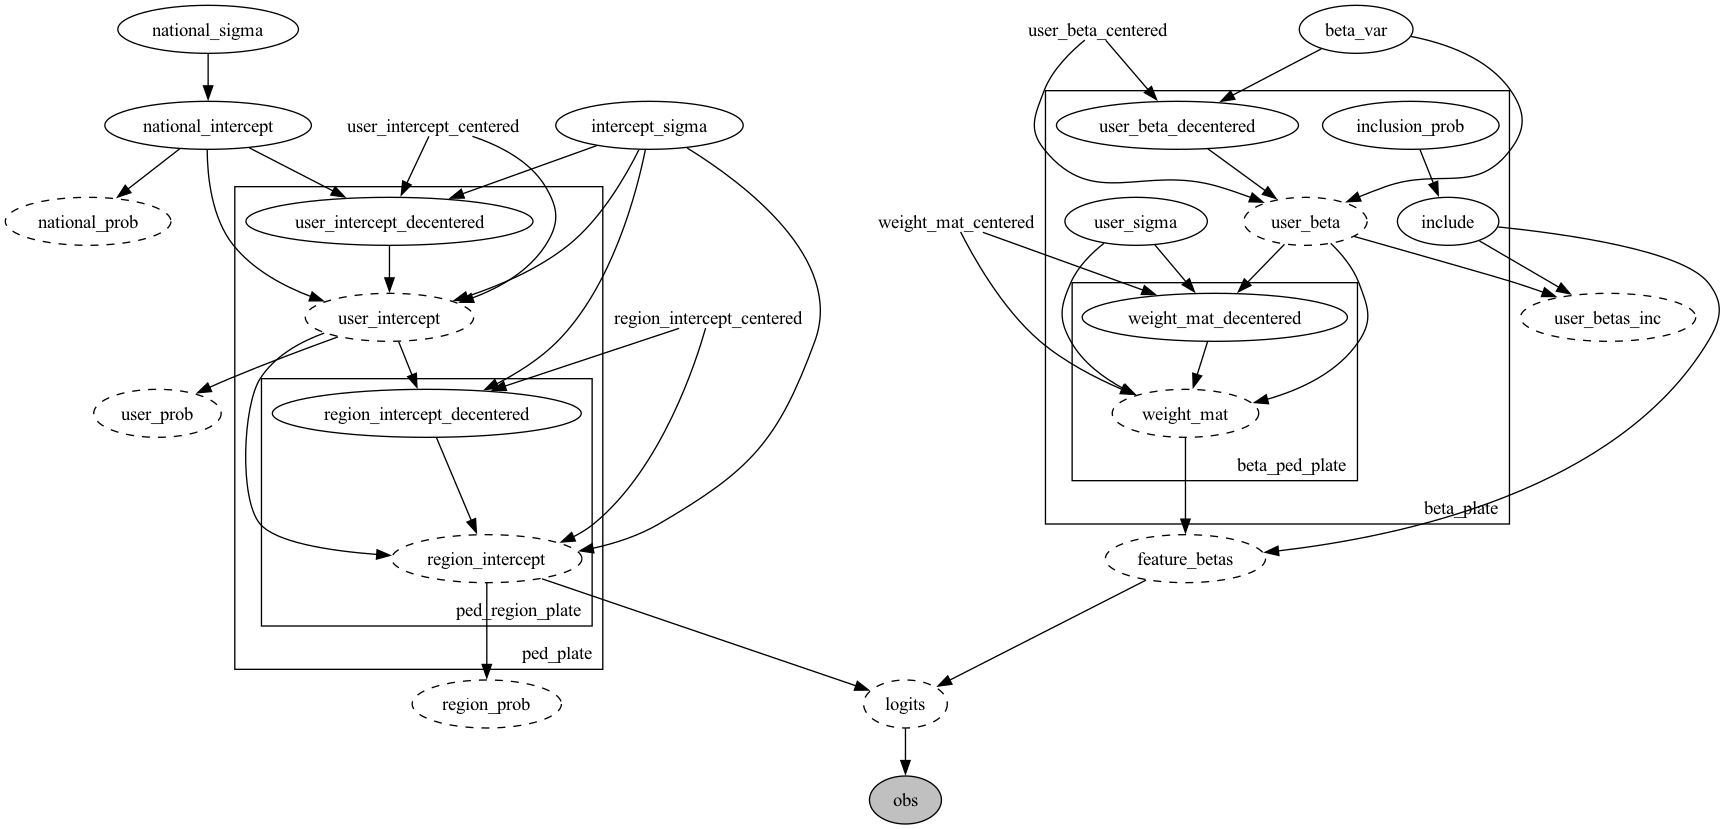
\includegraphics[width=\textwidth]{images/model_graph.png}
        \caption{Graphical representation of the hierarchical logistic regression model.}
        \label{fig:model_graph}
    \end{figure}


\begin{figure}[h]
    \centering
    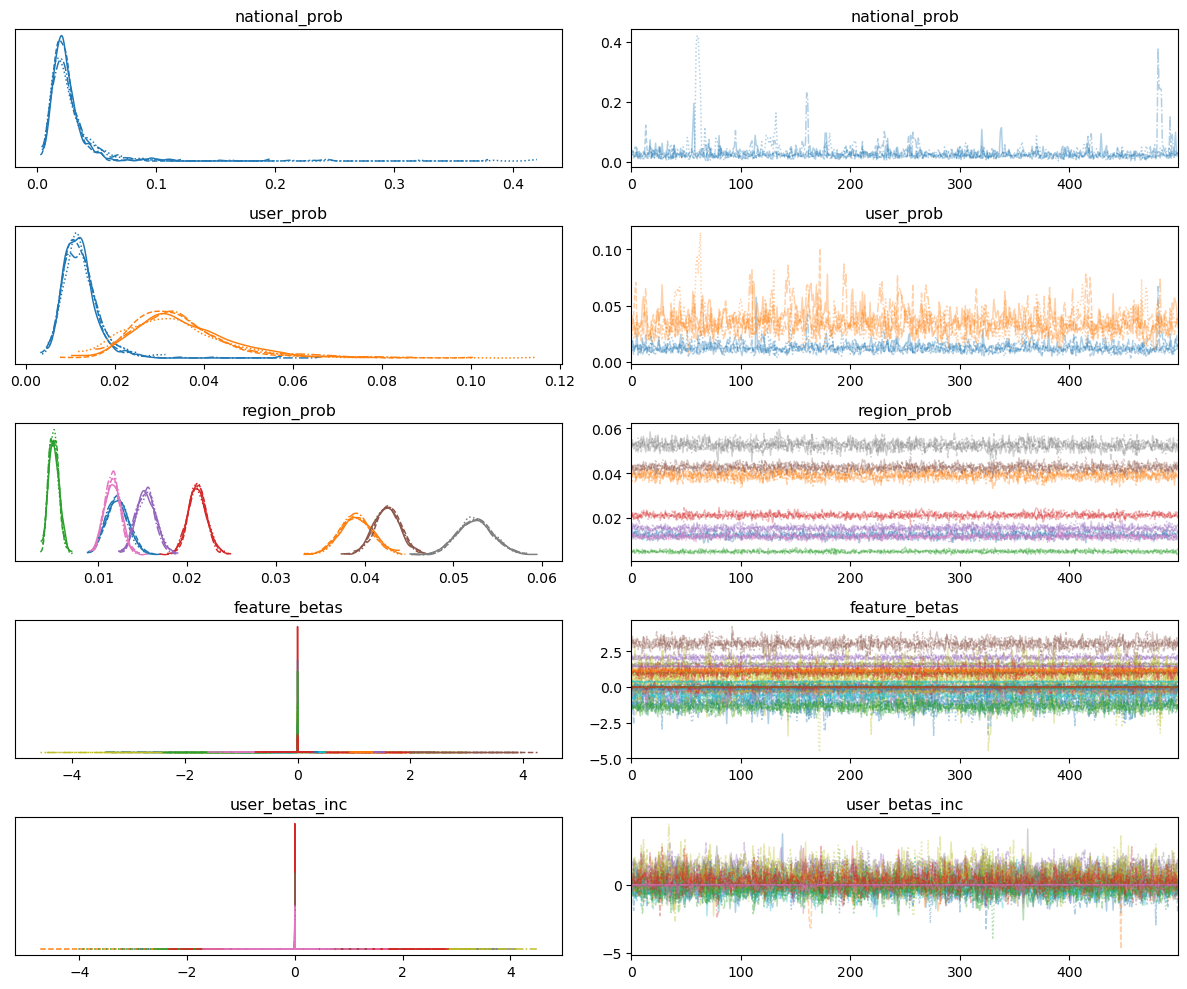
\includegraphics[width=\textwidth]{images/traceplot.png}
    \caption{Traceplot for all variables of interest. Note that there are no divergences and good mixing across all
        chains, indicating that the model has converged across all levels of the hierarchy without major issues. 
        The "spikes" in the probability distribution at 0 is indicative of the model averaging approach, and several 
        variables which are never selected have close to infinite probability density of at 0, thus compress the y-axis
        of the plot, hiding the overall effect of the other features.}
    \label{fig:traceplot}
\end{figure}


\begin{figure}[h]
    \centering
    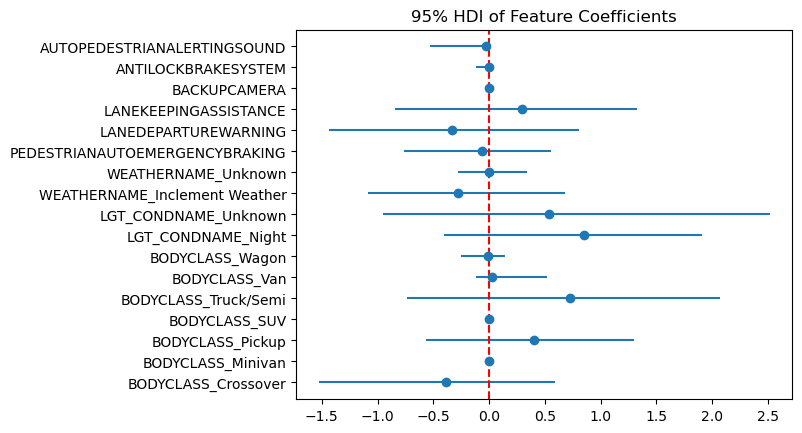
\includegraphics[width=\textwidth]{images/all_users_coefficients.png}
    \caption{Parent-level feature coefficients for variables of interest.}
    \label{fig:all_users}
\end{figure}


\begin{figure}[h]
    \centering
    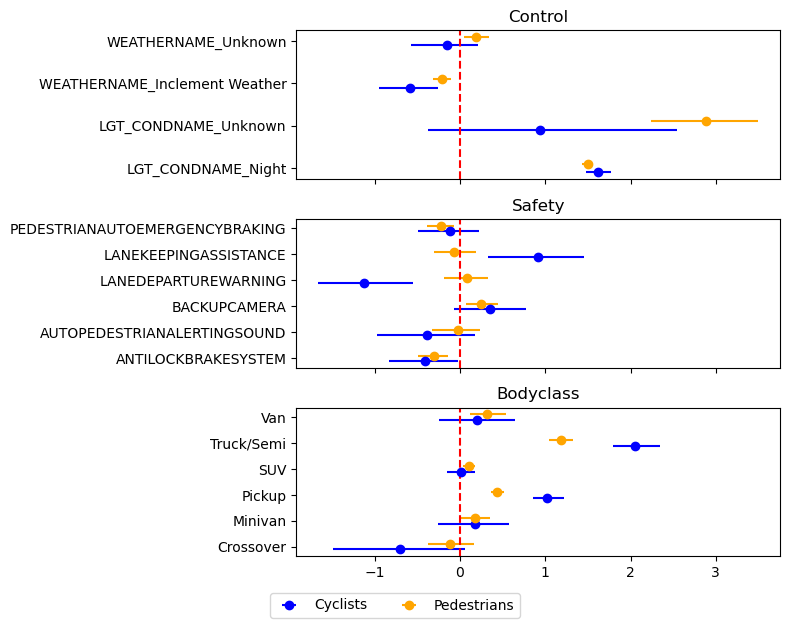
\includegraphics[width=\textwidth]{images/feature_coefficients.png}
    \caption{Feature coefficients for all variables of interest. The coefficients represent the change in the log-odds,
        and error bars represent the 95\% HDI interval.}
    \label{fig:coefficients}
\end{figure}


\begin{figure}[h]
    \centering
    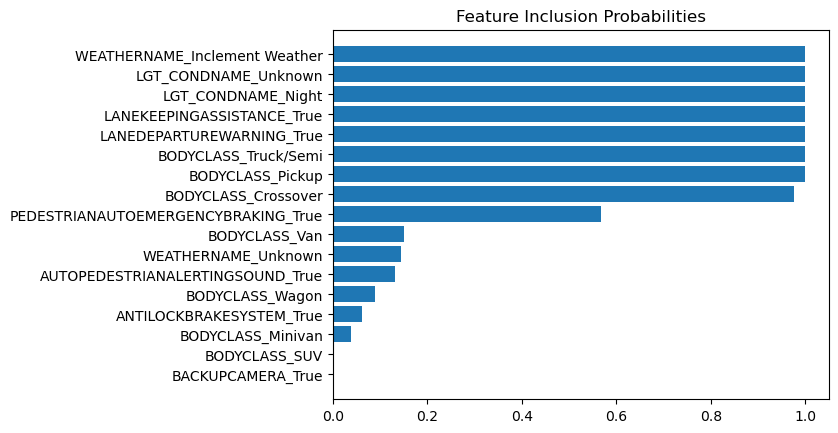
\includegraphics[width=\textwidth]{images/inclusion_probs.png}
    \caption{Probability of inclusion in the linear model for a particular coefficient.}
    \label{fig:inclusion_probs}
\end{figure}

\begin{figure}[h]
    \centering
    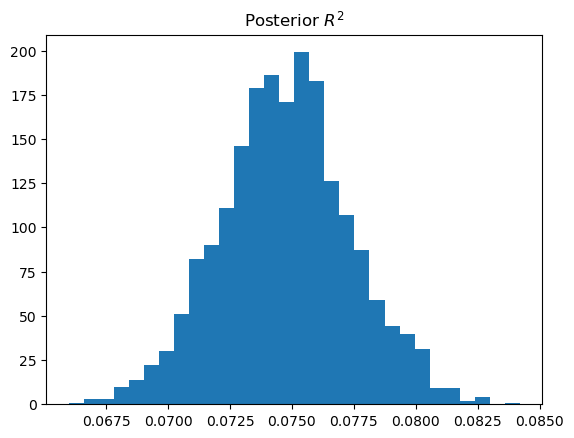
\includegraphics[width=\textwidth]{images/R2_dist.png}
    \caption{Distribution of $R^2$ for our model based on posterior samples, implemented as outlined by Gelman et. al.}
    \label{fig:r2_dist}
\end{figure}

\begin{figure}[h]
    \centering
    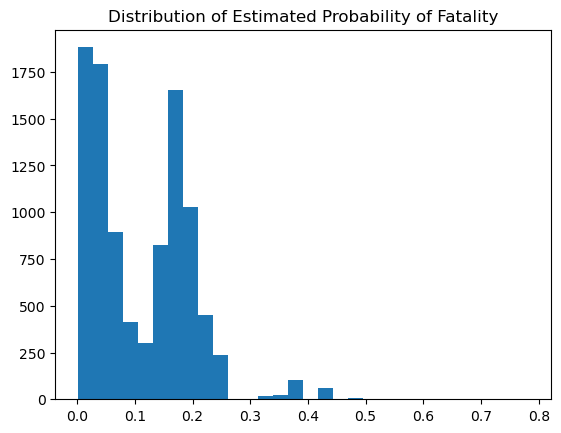
\includegraphics[width=\textwidth]{images/prob_dist.png}
    \caption{Distribution of estimated proabilities of fatalities for all crashes in our dataset.}
    \label{fig:prob_dist}
\end{figure}



\clearpage

\printbibliography

\end{document}



%%% Local Variables:
%%% mode: latex
%%% TeX-master: t
%%% End:
